\documentclass{article}
\usepackage[english,german]{babel}
\usepackage{graphicx}
\usepackage{amssymb}
\usepackage[utf8]{inputenc}
\usepackage{amsmath}
\usepackage{hyperref}

\begin{document}

\title{Hausarbeit SME-PHY-B: Wahlthema 2 - Fitnesszähler}
\author{Joel Ewig}
\date{\today}
\maketitle
\clearpage

\begin{abstract}
Es sollen sensorbasiert ähnlich einer Fitnessuhr verschiedene Sportübungen sowie deren Anzahl erkannt werden.
Benutzt werden sollen der Beschleunigungssensor und das Gyroskop des IMU-6050.\\
Mein Lösungsansatz gliedert sich in mehrere Stufen:
die Rohdaten aus dem IMU-6050 sollten durch einen mehrdimensionalen Kalman-Filter bereinigt werden.
Die bereinigten Daten werden mit dem K-Means Algorithmus geclustert um sie in Beobachtungen zu verarbeiten.
In der Lernphase wird mit diesen Beobachtungen pro Übung ein Hidden Markov Model erlernt.
In der folgenden Detektionsphase werden die empfangenen Daten ebenfalls geclustert und die Beobachtungen an alle Hidden Markov Modelle weitergegeben.
Das Hidden Markov Modell, welches die höchste Wahrscheinlichkeit für die Emittierung der beobachteten Folge bestimmt, gilt als Erkenner und die zugehörige Übung wird als ausgeführt behandelt.
\end{abstract}
\clearpage

\tableofcontents
\clearpage

\section{Konzept}
\label{sec:concept}
Hier soll die Idee, nach der vorgegangen wird, erläutert werden.
Genauere Angaben zur Sensorik sind in Kapitel \ref{sec:sensors}.
Die Umsetzung eines Kalman-Filters und warum dieser hier nicht umgesetzt wird, sind in Kapitel \ref{sec:kalman} zu finden.
Eine Erklärung zur Funktionsweise des Baum-Welch Algorithmus findet sich in Kapitel \ref{sec:BaumWelch}.
Abschließend wird eine Evaluierung auf Grundlage von Experimenten in Kapitel \ref{sec:evaluation} gezeigt.\\
Der hier betrachtete Ansatz nutzt in der Praxis zwei Phasen.
In der ersten Phase, der Lernphase, wird die Anzahl der zu erkennenden Übungen sowie für jede Übung eine Anzahl an Ausführungen festgelegt.
Nachdem diese durchgeführt wurden und fertig verarbeitet wurden, ist die Lernphase beendet.
In der Detektionsphase wird eine Anzahl an zu erkennenden Ausführungen festgelegt.
Nachdem diese durchgeführt wurden, wird das Ergebnis der Detektion ausgegeben und die Detektionsphase ist beendet.

\subsection{Lernphase}
Die einkommenden 6-dimensionalen Daten werden wie oben beschrieben mit einem K-Means geclustert.
Der K-Means (\cite{SklearnClusterKMeans2021}) wird auf den kompletten Trainingsdaten initialisiert, also unabhängig von den ausgeführten Übungen.
Jeder Punkt bekommt dadurch einen Clusternamen zugewiesen, umgesetzt als Nummer, welche weitergegeben werden.
Die Clusternummern sind die diskreten Beobachtungen die als Eingabe für das Lernen der Hidden Markov Modelle dienen.\\
Genutzt wird ein Hidden Markov Modell $(\pi, p, q)$ nach \cite{rabinerTutorialHiddenMarkov2001} mit:
\begin{enumerate}
\item $\pi: Z \rightarrow [0,1]$ für die initialen Wahrscheinlichkeiten der Zustände in $Z$
\item $p: Z \times Z \rightarrow [0,1]$ für die Übergangswahrscheinlichkeiten zwischen den Zuständen in $Z$
\item $q: Z \times B \rightarrow [0,1]$ für die Beobachtungswahrscheinlichkeiten für Beobachtung $B$ in den Zuständen in $Z$
\end{enumerate}
Ein Hidden Markov Modell für eine Übung wird wie folgt trainiert:\\
Zuerst werden die Emissionswahrscheinlichkeiten und die Übergänge zwischen den versteckten Zuständen zufällig initialisiert, konkret wird also $\pi$ mit Zufallszahlen im Intervall $[0,1]$ gefüllt.
Anschließend werden die genannten Werte mittels des Baum-Welch Algorithmus an die in der Lernphase aufgenommenen Sequenzen angepasst (mehr dazu in Kapitel \ref{sec:BaumWelch}).
Die Hidden Markov Modelle werden mehrfach initialisiert, um die Wahrscheinlichkeit nicht über ein lokales Optimum hinauszukommen zu vermindern.
Es wird das Modell gewählt, welches die größte Wahrscheinlichkeit bei der Erkennung der bekannten Übungen aufweist.
Durch die geringe Anzahl an Lerndaten wird hier keine Mindestwahrscheinlichkeit gesetzt, da dazu zu wenig Trainingsdaten vorhanden sind.
In den durchgeführten Experimenten hat sich kein Wert als stabil erwiesen, da hier versucht wurde mit möglichst wenigen Ausführungen auszukommen.
Dadurch bleibt der Trainingsdatenumfang relativ gering (mehr dazu in Kapitel \ref{sec:evaluation}).

\subsection{Detektionsphase}
In der Detektionsphase werden die empfangenen Daten mit dem K-Means aus der Lernphase geclustert.
Der K-Means ist eingefroren, das heißt die Clustermittelpunkte bleiben so wie sie in der Lernphase bestimmt wurden.\\
Die Beobachtungen einer Durchführung werden allen Hidden Markov Modelle zugeführt, diese geben die Emissionswahrscheinlichkeit für die beobachtete Sequenz aus.
Es wird die Übung erkannt, dessen zugehöriges Hidden Markov Modell die höchste Wahrscheinlichkeit für die Emission der beobachteten Sequenz ausgibt.

\subsection{Beispiel}
Es folgt ein Beispiel für eine typische Ausführung in der Detektionsphase:\\
Während der Ausführung einer Übung werden die Daten des Gyroskops und des Beschleunigungssensors erfasst.
Für 5 Zeitschritte haben die Gyroskopdaten folgende Form:
\begin{align*}
\left[\begin{array}{rrrrr}
g_{1}^1 & g_{1}^2 & g_{1}^3 & g_{1}^4 & g_{1}^5 \\
g_{2}^1 & g_{2}^2 & g_{2}^3 & g_{2}^4 & g_{2}^5 \\
g_{3}^1 & g_{3}^2 & g_{3}^3 & g_{3}^4 & g_{3}^5 \\
\end{array}\right]
\end{align*}
und die des Beschleunigungssensors folgende Form:
\begin{align*}
\left[\begin{array}{rrrrr}
a_{1}^1 & a_{1}^2 & a_{1}^3 & a_{1}^4 & a_{1}^5 \\
a_{2}^1 & a_{2}^2 & a_{2}^3 & a_{2}^4 & a_{2}^5 \\
a_{3}^1 & a_{3}^2 & a_{3}^3 & a_{3}^4 & a_{3}^5 \\
\end{array}\right]
\end{align*}
Diese werden mit einem mehrdimensionalen Kalman-Filter (Kapitel \ref{sec:kalman}) bereinigt und wie folgt zusammengeführt:
\begin{align*}
\left[\begin{array}{rrrrr}
a_{1}^1 & a_{1}^2 & a_{1}^3 & a_{1}^4 & a_{1}^5 \\
a_{2}^1 & a_{2}^2 & a_{2}^3 & a_{2}^4 & a_{2}^5 \\
a_{3}^1 & a_{3}^2 & a_{3}^3 & a_{3}^4 & a_{3}^5 \\
g_{1}^1 & g_{1}^2 & g_{1}^3 & g_{1}^4 & g_{1}^5 \\
g_{2}^1 & g_{2}^2 & g_{2}^3 & g_{2}^4 & g_{2}^5 \\
g_{3}^1 & g_{3}^2 & g_{3}^3 & g_{3}^4 & g_{3}^5 \\
\end{array}\right]
\end{align*}
Die Spaltenvektoren dienen als Eingabe für den K-Means Clustering Algorithmus.
Dieser gibt für jeden Spaltenvektor das zugehörige Cluster $c$ aus:
\begin{align*}
\left[\begin{array}{r}
a_{1}^1\\
a_{2}^1\\
a_{3}^1\\
g_{1}^1\\
g_{2}^1\\
g_{3}^1\\
\end{array}\right]
\rightarrow c_1
\end{align*}
Die Sequenz der Clusternamen dient als Eingabe in $n$ Hidden Markov Modelle, $n$ ist dabei die Anzahl der Übungen, die erkannt werden sollen.
Die Hidden Markov Modelle geben eine Emissionswahrscheinlichkeit für die beobachtete Folge an:
\begin{align*}
\left[c_1, c_2, c_3, c_4, c_5\right] \rightarrow p_1, ..., p_n
\end{align*}
Aus den Emissionswahrscheinlichkeiten $p$ wird die größte gewählt.
Die zum gewählten Hidden Markov Modell gehörende Übung gilt als erkannt.

\newpage
\section{Sensorik}
\label{sec:sensors}
Auf dem Arduino werden die Daten des Beschleunigungssensors und des Gyroskop aus dem IMU ausgelesen.
Das Gyroskop sowie der Beschleunigungssensor werden dem im Datenblatt beschriebenem Selbsttest unterzogen.
Dieser soll feststellen, ob die Sensoren noch funktionsfähig sind.
Die zugehörigen Daten werden über die serielle Schnittstelle an ein Pythonskript übermittelt, welches die zugehörigen Rechnungen vornimmt und bei Nichtbestehen des Selbsttests das Programm beendet.\\
Der Aufbau des Arduinos ist in Abbildung \ref{fig:arduino} zu sehen.
\begin{figure}[htbp]
\centering
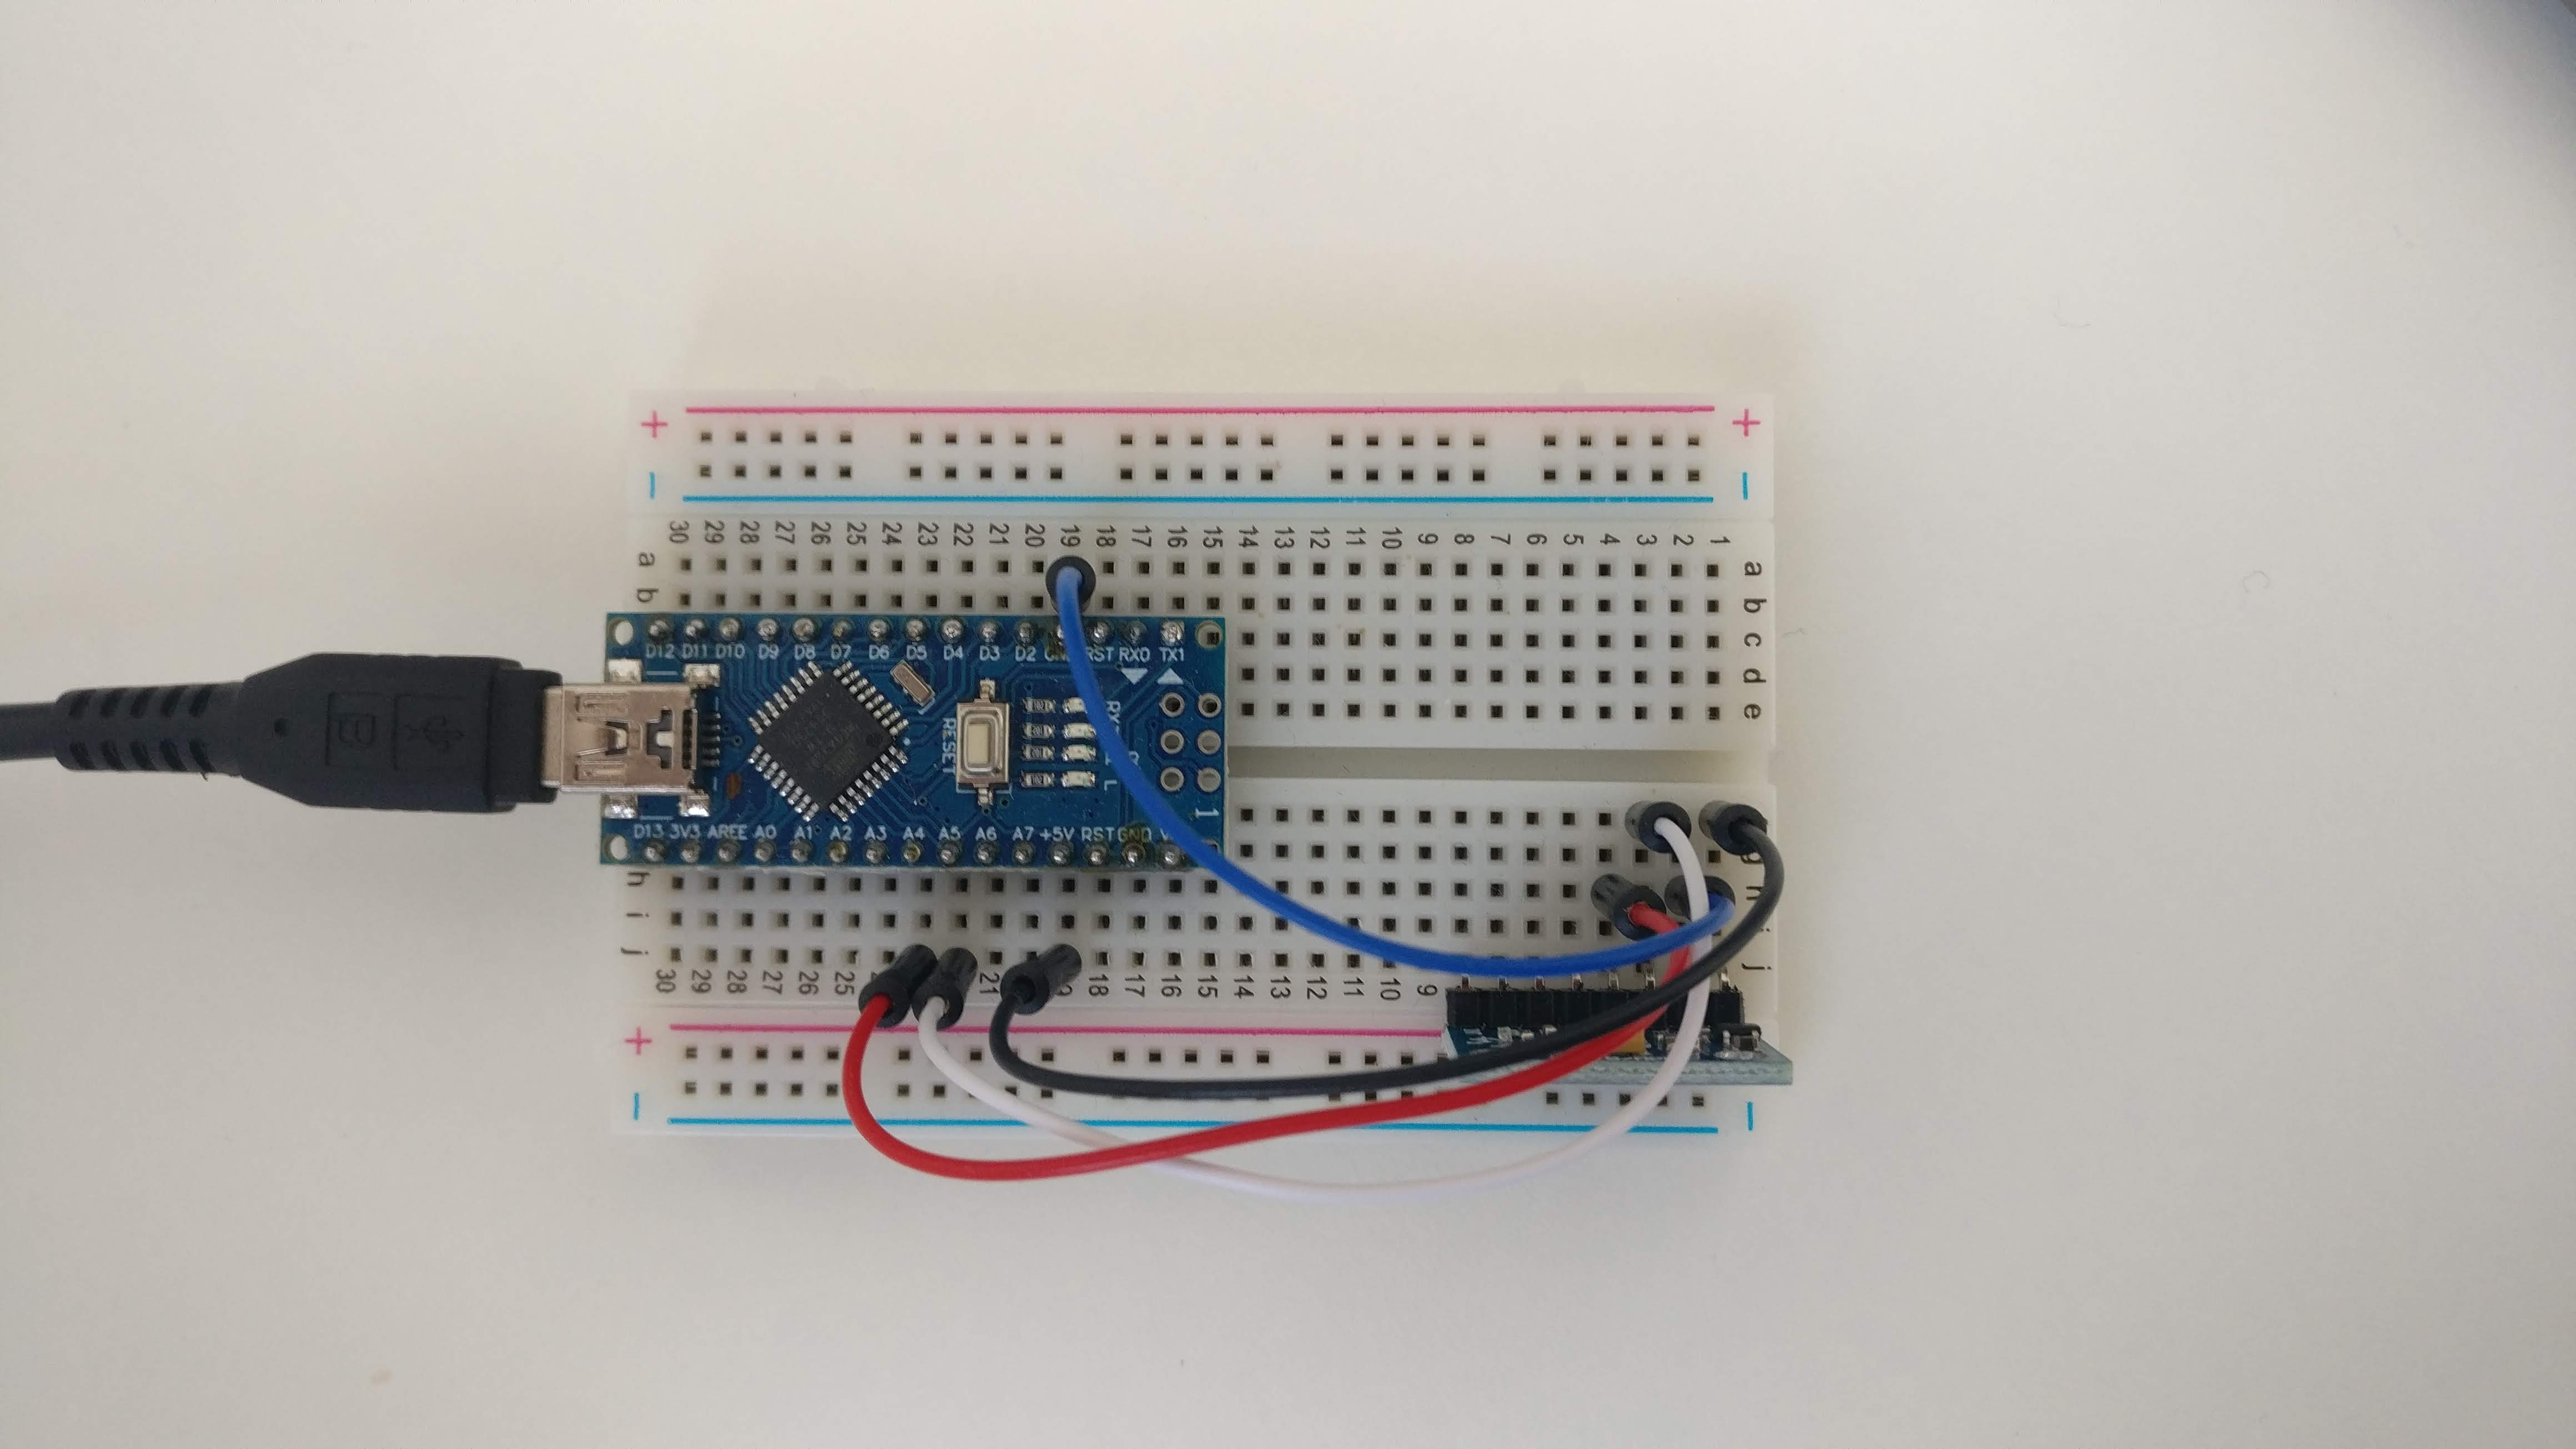
\includegraphics[width=\textwidth]{figures/aufbau.jpg}
\caption{Aufbau und Verbindungen des Arduinos und des genutzten Sensors.}
\label{fig:arduino}
\end{figure}\\


\section{Mehrdimensionaler Kalman-Filter}
\label{sec:kalman}
Hier wird aus Zeitgründen auf einen Kalman-Filter verzichtet, da dieser die Ergebnisse zwar verbessern würde, allerdings nicht unbedingt notwendig ist.
Mit einem solchen Kalman-Filter wäre die Erkennung vermutlich robuster, da mit bereinigten Daten \glqq engere\grqq{} Cluster zu erwarten wären.
Ein solcher Filter würde wie folgt aussehen:
\begin{align*}
X^{[t+1]} &= A^{[t]}X^{[t]} + B^{[t]}u^{[t]} + C^{[t]} + \epsilon^{[t]}\\
\left[\begin{array}{r}
a_{1}\\
a_{2}\\
a_{3}\\
g_{1}\\
g_{2}\\
g_{3}\\
\end{array}\right]^{[t+1]}
&= A^{[t]} \left[\begin{array}{r}
a_{1}\\
a_{2}\\
a_{3}\\
g_{1}\\
g_{2}\\
g_{3}\\
\end{array}\right]^{[t]}
+ B^{[t]}\left[\begin{array}{r}
ra_{1}\\
ra_{2}\\
ra_{3}\\
rg_{1}\\
rg_{2}\\
rg_{3}\\
\end{array}\right]^{[t]}
+ C^{[t]} + \epsilon^{[t]}
\end{align*}
Dabei müssen $A^{[t]}$, $B^{[t]}$ und $C^{[t]}$ gesetzt und experimentell überprüft werden.
Hier modelliert $\epsilon^{[t]}$ das Messrauschen und ist damit bei der Implementierung nicht zu beachten.
Es darf allerdings nicht vergessen werden, dass der Kalman-Filter nur ein Zustands\textbf{schätzer} ist.

\newpage
\section{Baum-Welch Algorithmus}
\label{sec:BaumWelch}
Der Baum-Welch Algorithmus wendet den Maximum-Likelihood Algorithmus auf Hidden Markov Modelle an.
Genutzt wird ein Hidden Markov Modell $(\pi, p, q)$ mit:
\begin{enumerate}
\item $\pi: Z \rightarrow [0,1]$ als inititale Wahrscheinlichkeiten für die Zustände $Z$
\item $p: Z \times Z \rightarrow [0,1]$ als Übergangswahrscheinlichkeiten zwischen den Zuständen $Z$
\item $q: Z \times B \rightarrow [0,1]$ als Beobachtungswahrscheinlichkeiten für die Beobachtung $B$ in den Zuständen $Z$
\end{enumerate}
In der hier genutzten Implementierung (\cite{HmmlearnHmmlearn2021}) sind $p$ und $q$ als Matrizen umgesetzt.
Diese werden zu Beginn mit zufälligen Werten initialisiert.
Im ersten Schritt werden die Wahrscheinlichkeiten mit den aktuellen Parametern ermittelt.
Die Idee hinter dem Baum-Welch Algorithmus ist es, die Übergänge, die der wahrscheinlichste Pfad durch das Hidden Markov Modell nutzt, wahrscheinlicher zu machen.\\
Die nachfolgende Passage orientiert sich an der Erklärung in \cite{wunschBaumWelchAlgorithmusFu2001}.
Für eine beobachtete Sequenz $O = {o_1, .., o_T}$ heißt das, dass $\pi$ in der nächsten Iteration zu $\tilde{\pi}$ wird und berechnet sich wie folgt:
\[
\tilde{\pi_i} = \gamma_i(1)
\]
$\gamma_i(t)$ ist die erwartete Häufigkeit, sich in Zustand $i$ zum Zeitpunkt $t$ aufzuhalten.
Diese ergibt sich aus:
\[
\gamma_i(t) = \frac{\alpha_i(t)\beta_i(t)}{\sum_{j=1}^{N}\alpha_j(t)\beta_j(t)}
\]
$\alpha$ und $\beta$ können rekursiv ermittelt werden über:
\begin{align*}
\alpha_i(1) &= \pi_iq_i(o_1) \\
\alpha_j(t+1) &= \sum_{i=1}^{N}\alpha_i(t)p(i, j)q_j(o_{t+1})\\
\beta_i(T) &= 1 \\
\beta_i(t) &= \sum_{j=1}^{N}p(i, j)q_j(o_{t+1})\beta_j(t+1)
\end{align*}
Dann werden $p$ und $q$ angepasst mit:
\begin{align*}
p(i, j) &= \frac{\text{Anzahl der Übergänge von i nach j}}{\text{Anzahl der Übergänge von i zu einem beliebigen Zustand}}\\
\\
q_i(k) &= \frac{\text{Anzahl der Zeitschritte in i in denen k beobachtet wurde}}{\text{Anzahl der Zeitschritte in i}}
\end{align*}
Diese Operationen werden so lange ausgeführt bis sich keiner der Werte um mehr als ein Mindestwert (hier: 0,01) verändert oder die festgelegte Höchstanzahl an Iterationen (hier: 100) erreicht ist.

\newpage
\section{Evaluierung}
\label{sec:evaluation}
Im Folgenden werden vor allem Experimente mit dem bestehenden Ansatz und verschiedenen Parametern betrachtet.
Es wurde beobachtet, dass Übungen, die keine oder wenig Bewegung des Arduinos umfassen, die Erkennungsleistung maßgeblich verschlechtern.
Es liegt die Vermutung nahe, dass die meisten Übungen im Stillstand beginnen, enden oder einen \glqq Umkehrpunkt\grqq{} beinhalten.
Damit wird meist ein Zeitschritt erfasst, welcher eine Beschleunigung nahe null aufweist.
Man kann diesen Sprung in den folgenden Diagrammen auch beobachten: der Sprung in der Erkennungsleistung von Abbildung \ref{fig:drei} auf Abbildung \ref{fig:vier} liegt unter anderem daran, dass die vierte Übung viel Stillstand beinhält.\\
Die folgenden Diagramme wurden mit verschieden vielen Übungen, die erkannt werden sollen erstellt.
Auf der Hochachse ist der Anteil an richtig erkannten Übungen aufgetragen.
Auf den anderen Achse jeweils die Clusteranzahl und die Ausführungsanzahl während der Trainingsphase.
Hier werden nicht die üblichen Maße Precision und Recall genutzt, da wie oben beschrieben keine feste Mindestwahrscheinlichkeit festgelegt werden konnte und damit ein Nichterkennen nicht scharf definiert werden kann.
Das liegt daran, dass das entsprechende Hidden Markov Modell zwar eine hohe Wahrscheinlichkeit ausgeben kann, ein Fehlerhaftes jedoch eine noch größere, was aber nichts über das betrachtete Modell aussagt.\\
Die Daten zu den Schaubildern bauen aufeinander auf, die Ausführungen für die Übungen sind immer dieselben.
Es werden nur mehr Übungen oder Ausführungen betrachtet.
Die gesehenen Ausführungen sind also entlang einer Linie immer die selben.
Die Hidden Markov Modelle haben jeweils 5 versteckte Zustände, was sich in Experimenten als bester Kompromiss zwischen Lernzeit und Erkennungsleistung herausgestellt hat.
\medskip
\begin{figure}[h]
\centering
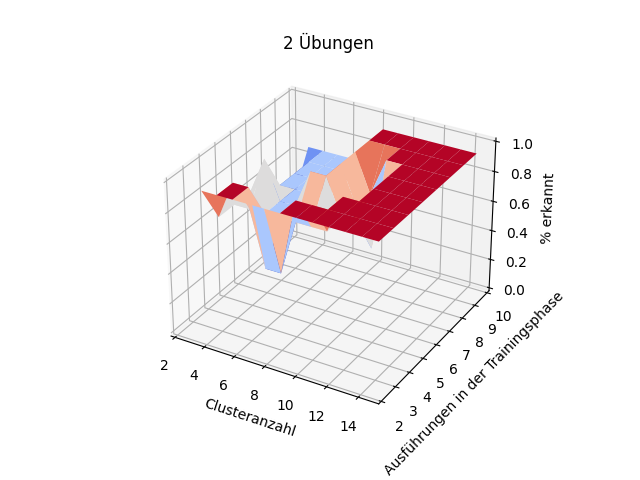
\includegraphics[width=0.7\textwidth]{figures/2_graph.png}
\caption{Diagramm für 2 verschiedene Übungen}
\label{fig:zwei}
\end{figure}\\
Bei der Unterscheidung von 2 Übungen (Abbildung \ref{fig:zwei}) ist die Erkennungsleistung im Allgemeinen sehr hoch, aber ein höheres $k$, also eine höhere Anzahl an Clustern, trennt hier die Übungen schärfer voneinander.
Die Anzahl an Ausführungen spielt in diesem Fall dagegen eine eher untergeordnete Rolle für die Erkennungsleistung.
\medskip
\begin{figure}[h]
\centering
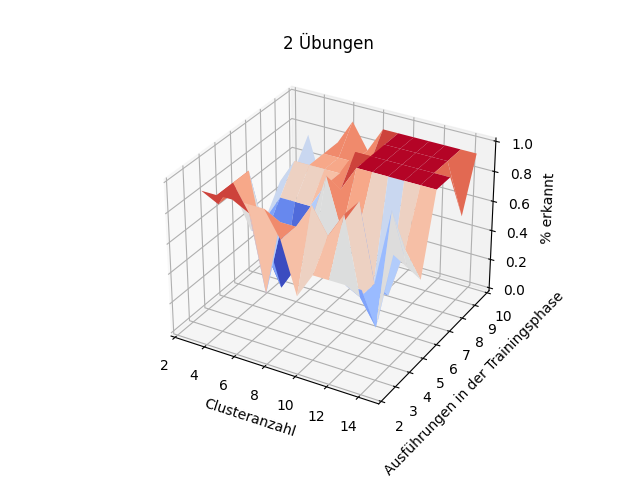
\includegraphics[width=0.7\textwidth]{figures/3_graph.png}
\caption{Diagramm für 3 verschiedene Übungen}
\label{fig:drei}
\end{figure}\\
In Abbildung \ref{fig:drei} wird deutlich, dass die Anzahl an Ausführungen mehr ins Gewicht fällt.
Auch hier ist wieder zu erkennen, dass ein etwas größeres $k$ bessere Ergebnisse erzielt.
Dieses sollte man jedoch auch nicht zu hoch wählen, da sonst einzelne, tatsächliche Cluster aufzuteilen welche das Hidden Markov Modell dann als gleichwertig erlernen muss.
Außerdem wird damit auch das Hidden Markov Modell umfangreicher und mehr Ausführungsdaten werden benötigt um gute Ergebnisse zu erzielen.\\
\medskip
\begin{figure}[htbp]
\centering
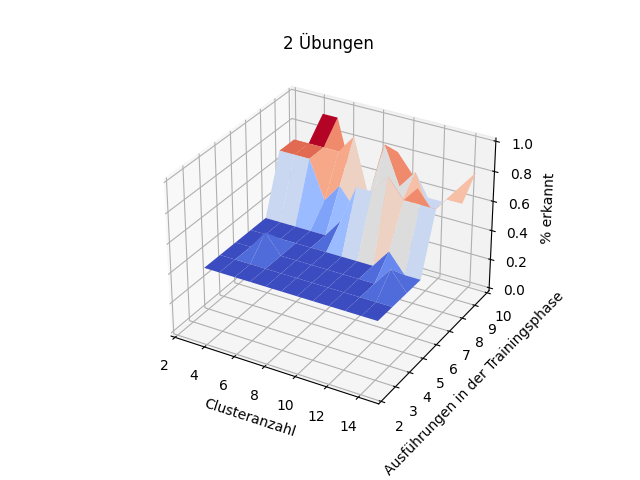
\includegraphics[width=0.7\textwidth]{figures/4_graph.png}
\caption{Diagramm für 4 verschiedene Übungen}
\label{fig:vier}
\end{figure}\\
Für die Unterscheidung von 4 Übungen (Abbildung \ref{fig:vier}) ist der oben erwähnte negative Sprung zu sehen, da die vierte Übung weniger Bewegung umfasst.
Der bisher ersichtliche Vorteil von mehr Clustern scheint sich zu verkleinern, ist aber noch erkennbar.
Eine höhere Ausführungsanzahl scheint hier den klaren Vorteil zu bringen.\\
\medskip
\begin{figure}[htbp]
\centering
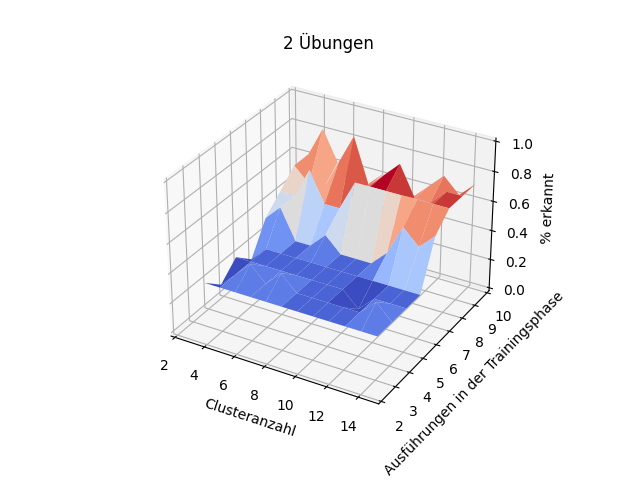
\includegraphics[width=0.7\textwidth]{figures/5_graph.png}
\caption{Diagramm für 5 verschiedene Übungen}
\label{fig:fuenf}
\end{figure}\\
Mit 5 Übungen als Grundlage (Abbildung \ref{fig:fuenf}) verfestigt sich der bisherige Trend, dass mehr Ausführungen zu deutlich besseren Ergebnissen führt.
Die Clusteranzahl bietet keinen deutlichen Vorteil mehr.\\
Abschließend lässt sich feststellen, dass mehr Ausführungen bei mehr Übungen die Erkennungsleistung deutlich steigern.
Darüber hinaus sollte auch immer ein $k$ gewählt werden, das nicht zu klein ist, vor allem für wenige Übungen.\\

Als Ausgangspunkt empfiehlt es sich $k=5$ zu setzen, $5$ versteckte Zustände und $5$ Ausführungen zu nutzen.
Diese Parameter können dann natürlich je nach Bedarf angepasst werden.

\newpage
\addcontentsline{toc}{section}{Bibliographie}
\bibliographystyle{apalike}
\bibliography{phyb}

\end{document}
